\def\mySecNum{10.3}
\mySection{\mySecNum~Two or more binomial periods}
%-------------- start slide -------------------------------%{{{ 1
\begin{frame}[fragile,t]
\begin{center}
	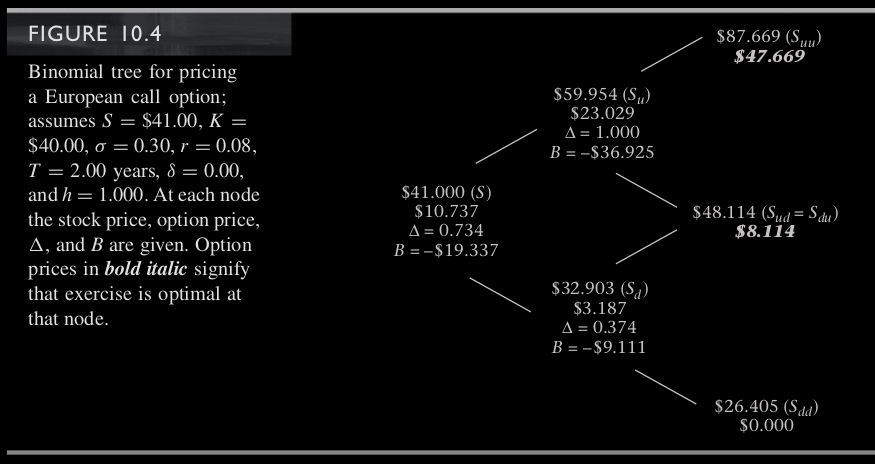
\includegraphics[scale=0.3]{figs/Figure-10-4.png}
\end{center}
\end{frame}
%-------------- end slide -------------------------------%}}}
%-------------- start slide -------------------------------%{{{ 1
\begin{frame}[fragile,t]
	\centering

	Some observations:
	\bigskip

	\begin{itemize}
		\item The option price is greater for the 2-year than for the 1-year option
		\item The option was priced by working \textcolor{cyan}{backward} through the binomial tree.
		\item The option’s $\Delta$ and $B$ are different at different nodes. At a given point in time, $\Delta$ increases to 1 as we go further into the money
		\item Permitting early exercise would make no difference. At every node prior to expiration, the
			option price is greater than $S – K$; hence, we would not exercise even if the option had been
			American.
	\end{itemize}
\end{frame}
%-------------- end slide -------------------------------%}}}
%-------------- start slide -------------------------------%{{{ 1
\begin{frame}[fragile,t]
	Dividing the time to expiration into more periods allows us to generate a more realistic tree with
	a larger number of different values at expiration.
\end{frame}
%-------------- end slide -------------------------------%}}}
%-------------- start slide -------------------------------%{{{ 1
\begin{frame}[fragile,t]
\begin{center}
	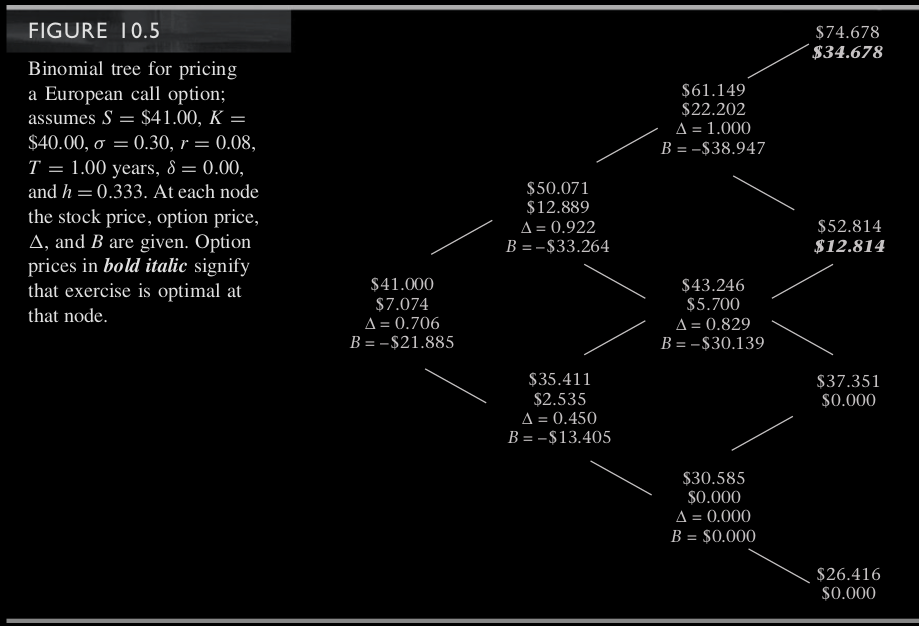
\includegraphics[scale=0.25]{figs/Figure-10-5.png}
\end{center}
\end{frame}
%-------------- end slide -------------------------------%}}}
